\documentclass{report}
\usepackage[T1]{fontenc} % Fontes T1
\usepackage[utf8]{inputenc} % Input UTF8
\usepackage[backend=biber, style=ieee]{biblatex} % para usar bibliografia
\usepackage{csquotes}
\usepackage[portuguese]{babel} %Usar língua portuguesa
\usepackage{blindtext} % Gerar texto automaticamente
\usepackage[printonlyused]{acronym}
\usepackage{hyperref} % para autoref
\usepackage{graphicx}

\usepackage{listings}
\usepackage{color}

\definecolor{dkgreen}{rgb}{0,0.6,0}
\definecolor{gray}{rgb}{0.5,0.5,0.5}
\definecolor{mauve}{rgb}{0.58,0,0.82}

\lstset{frame=tb,
  language=Python,
  aboveskip=3mm,
  belowskip=3mm,
  showstringspaces=false,
  columns=flexible,
  basicstyle={\small\ttfamily},
  numbers=none,
  numberstyle=\tiny\color{gray},
  keywordstyle=\color{blue},
  commentstyle=\color{dkgreen},
  stringstyle=\color{mauve},
  breaklines=true,
  breakatwhitespace=true,
  tabsize=3
}

\bibliography{bibliografia}


\begin{document}
%%
% Definições
%
\def\titulo{Relatório AP2}
\def\data{19 de Abril de 2018}
\def\autores{Daniel Correia, Pedro Valente}
\def\autorescontactos{(88753) dcorreia@ua.pt, (88858) pedro.valente@ua.pt}
\def\departamento{Departamento de Eletrónica, Telecomunicações e Informática}
\def\empresa{Universidade de Aveiro}
\def\logotipo{ua.pdf}
%
%%%%%% CAPA %%%%%%
%
\begin{titlepage}

\begin{center}
%
\vspace*{50mm}
%
{\Huge \titulo}\\ 
%
\vspace{10mm}
%
{\Large \empresa}\\
%
\vspace{10mm}
%
{\LARGE \autores}\\ 
%
\vspace{30mm}
%
\begin{figure}[h]
\center
\includegraphics{\logotipo}
\end{figure}
%
\vspace{30mm}
\end{center}
%
\begin{flushright}

\end{flushright}
\end{titlepage}

%%  Página de Título %%
\title{%
{\Huge\textbf{\titulo}}\\
{\Large \departamento\\ \empresa}
}
%
\author{%
    \autores \\
    \autorescontactos
}
%
\date{\data}
%
\maketitle

\pagenumbering{roman}

%%%%%% Agradecimentos %%%%%%
% Segundo glisc deveria aparecer após conclusão...
\renewcommand{\abstractname}{Agradecimentos}
\begin{abstract}
Neste trabalho queremos agradecer a: 
\begin{itemize}
\item Professor de aula António Adrego
\item Prof. João Paulo Barraca pela disponibilidade de resposta relativos aos problemas com a sonda.
\end{itemize}
\end{abstract}


\tableofcontents
% \listoftables     % descomentar se necessário
% \listoffigures    % descomentar se necessário


%%%%%%%%%%%%%%%%%%%%%%%%%%%%%%%
\clearpage
\pagenumbering{arabic}

%%%%%%%%%%%%%%%%%%%%%%%%%%%%%%%%
\chapter{Introdução}
\label{chap.introducao}

Para este projeto foi proposta a criação de um cliente com a capacidade de aceder remotamente à sonda, registando os dados num ficheiro Comma Separated Values (CSV). 
Além disso, deverão ser apresentadas no terminal algumas indicações sobre a possibilidade (ou
necessidade) de se levar t-shirt, casaco, gorro ou outras peças de roupa.

Este cliente recebe os valores de temperatura, humidade e vento através de uma sonda, estes valores devem ser recebidos de forma automática e constante, de 10 em 10 segundos.

A comunicação com a sonda faz-se através de um socket Transmission Control Protocol
(TCP), na porta 8080 do servidor xcoa.av.it.pt, enviando-se comandos de texto
e recebendo-se objectos JavaScript Object Notation (JSON). 

O grupo decidiu também realizar uma interface gráfica para melhor verificação dos resultados do trabalho, esta pode ser acedida através da pasta "gui".



\chapter{Metodologia}
\label{chap.metodologia}
Neste capítulo explicaremos o código usado no trabalho, este está dividido por funções para mais fácil entendimento. Passaremos agora a explicar cada uma das funções.

\section{Connect \textunderscore tcp}
\begin{lstlisting}
def connect_tcp():
	tcp_s = socket.socket(socket.AF_INET, socket.SOCK_STREAM)
	tcp_s.bind( ("0.0.0.0", 0))	
	tcp_s.connect( ("xcoa.av.it.pt", 8080) )
	return tcp_s
\end{lstlisting}

Esta função cria o socket e liga-se ao servidor pot TCP.

\newpage

\section{Get\textunderscore key}
\begin{lstlisting}
def get_key(server):
	p = 1343270965545476954223465975446
	g = 46756894379
	a = (int)(random.random()*10)
	server.send(("CONNECT " + str(pow(g,a,p)) + "," +str(p) + "," + str(g) +"\n").encode("utf-8"))
	

	data = server.recv(4098)
	data = data.decode("utf-8")
	data = json.loads(data)
	token = data["TOKEN"]
	b = data["B"]
	X = pow(b,a,p)
	X = str(X).encode("utf-8")
	MD5 = hashlib.md5()
	MD5.update(X)
	X = MD5.hexdigest()
	X = X[0:16]
	
	return X, token

\end{lstlisting}

Esta função cria o valor "a" aleatório e envia para o servidor a instrução "CONNECT A,p,g".
De seguida recebe do servidor o "TOKEN" e o valor "B".
A partir deste valor "B" calcula a chave comum "X". 

\newpage

\section{Encode\textunderscore data}
\begin{lstlisting}
def encode_data(data, key):
	cipher = AES.new(key)
	

	lastBlockLen = len(data) % cipher.block_size
	if (lastBlockLen != cipher.block_size):
		p = cipher.block_size - len(data)
		data = data + chr(p)*p

	data = cipher.encrypt(data)
	data = base64.b64encode(data)+"\n".encode("utf-8")
	return data

\end{lstlisting}

Esta função encripta em AES e codifica em base64 uma mensagem passada como argumento.

\section{Get\textunderscore data}
\begin{lstlisting}
def get_data(server, key):
	cipher = AES.new(key)
	
	data = server.recv(4096)
	data = base64.b64decode(data)
	data = cipher.decrypt(data)
	p = data[len(data)-1]
	data = data[0:len(data)-p]
	return data

\end{lstlisting}

Esta função recebe dados do servidor, descodifica-os em base64 e desencripta-os com cifra AES.

\section{Create\textunderscore cvs}
\begin{lstlisting}
def create_csv(name):
	fout = open(name, 'w')
	writer = csv.DictWriter(fout, fieldnames=['WIND', 'HUMIDITY', 'TEMPERATURE'])
	writer.writeheader()
	return writer
\end{lstlisting}

Esta função cria um ficheiro CSV e imprime nele o cabeçalho com os parâmetros vento, humidade e temperatura, devolvendo o "writer" que permite mais tarde escrever os valores no ficheiro.

\section{write\textunderscore to\textunderscore csv}
\begin{lstlisting}
def write_to_csv(writer, data):
    writer.writerow(data)
\end{lstlisting}

Esta função escreve uma linha de dados(vento, humidade e temperatura) no CSV.


\section{write\textunderscore msg}
\begin{lstlisting}
def write_msg(wind, humi, temp):
	if(humi < 80 and temp > 10 and wind < 30):
		print("Esta bom tempo")
	else:
		print("O tempo nao esta muito bom")
		if(humi >= 80):
			print("Levar Guarda-Chuva")
		if(temp <= 10 or wind >= 30):
			print("Levar Casaco")
\end{lstlisting}

Esta função analisa os dados de vento, humidade e temperatura e imprime para o utilizador uma mensagem correspondente.

\newpage

\section{Initialize}
\begin{lstlisting}
def initialize():
	print("Aplicacao de monitorizacao do clima\n\n")
	
	print("A ligar ao servidor...\n")
	server = connect_tcp()
	print("Ligado.\n")
	print("A obter chave de encriptacao...\n")
	X, token = get_key(server)
	print("Chave obtida com sucesso\n")

	print("A pedir os dados ao servidor...\n")
	data = ("READ " + str(token))

	data = encode_data(data, X)
	server.send(data)


	writer = create_csv("data.csv")
	
	data = get_data(server, X).decode("utf-8")
	print("Servidor OK\n")
	print("Ctrl + c para terminar o programa\n\n")
	
	return (server, writer, X)
\end{lstlisting}

Esta função chama todas as funções de inicialização ("connect\textunderscore tcp", "get\textunderscore key", "create\textunderscore csv") e envia para o servidor a mensagem "READ TOKEN"  de forma a começar a receber os dados.

\newpage

\section{Main}
\begin{lstlisting}
def main():
	
	X = None
		
	while (X == None):	
		try:
			server, writer, X = initialize()
		except socket.gaierror:
			print("Nao foi possivel ligar ao servidor")
			exit(0)
		except:
			print("Ocureu um erro, o programa vai reiniciar\n\n\n")
	
	while 1:
		try:
			data = json.loads(get_data(server, X).decode("utf-8"))
			write_to_csv(writer, data)
			print("\n\nVento: " + str(data["WIND"]))
			print("Humidade: " + str(data["HUMIDITY"]))
			print("Temperatura: " + str(data["TEMPERATURE"]) + "\n")
			write_msg(data['WIND'], data['HUMIDITY'], data['TEMPERATURE'])
		except KeyboardInterrupt:
			exit()
		except:
			pass
		
main()
\end{lstlisting}

Esta função é a função principal do programa que inicializa o programa e contém um loop infinito que vai lendo os dados do servidor.


\chapter{Resultados}
\label{chap.resultados}

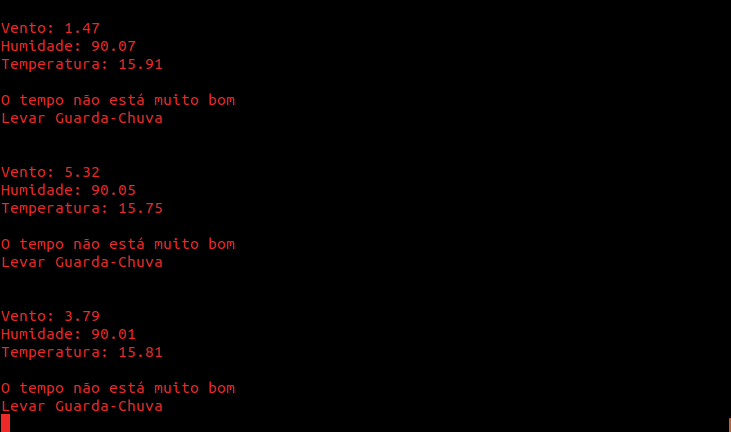
\includegraphics[scale=0.5]{Terminal}
\newline
\newline

\textbf{O projeto funciona como é suposto.} 


\chapter{Conclusões}
\label{chap.conclusao}
Com este trabalho consolidamos os nossos conhecimentos de Python, podendo prepararmon-nos melhor para o projeto final. \newline Usando também conhecimentos de documentos de texto, realizamos o projeto proposto com sucesso. 

\chapter*{Contribuições dos autores}
A contribuição dos autores é de 50\% para Daniel Correia e 50\% para Pedro Valente.


\end{document}
